\section{Ruta 3: Universidad de Ljubljana}

Ejecutamos la herramienta usando la dirección \texttt{www.uni-lj.si}, y al igual que en los demás casos con ráfagas de 100 paquetes y TTL máximo 30.

Realizamos un gráfico de la ruta obtenida usando una página de geolocalización por IP \cite{ip2location}, que se encuentra en la figura \ref{mapa3}.

\subsection{Análisis de la ruta obtenida}

Los paquetes hacen varios saltos en Buenos Aires (aunque algunos no responden podemos suponer que son en Buenos Aires), luego de lo cual hay un salto de Buenos Aires a Viena. Esto es anormal, ya que el único cable submarino que conecta Argentina y Europa llega a Portugal, el Atlantis-2 \cite{atlantis2}. Usando otras fuentes para geolocalización de IP vemos que la IP \texttt{185.70.203.22} del salto 8 podría en realidad estar localizada en Italia. Al igual que en la primera ruta creemos que esto se debe a la utilización del mismo cable Atlantis-2, y que esa IP podría estar en Portugal.

Luego hay algunos saltos más en Europa hasta llegar a destino. Hay un solo salto intercontinental en el mapa, que es el salto Buenos Aires-Viena (o bien Buenos Aires-Portugal), este salto es detectado correctamente, pero al igual que en experimentos anteriores hay muchos falsos positivos.

Observamos que el destino final de los paquetes no es la ciudad de Ljubljana, sino Nova Gorica que se encuentra a aproximadamente 100 kilómetros. Es posible que los servidores de la universidad se encuentren allí.

\subsection{Análisis de las predicciones de salto intercontinental}

En la tabla \ref{tabla3} vemos que la mayoría de los saltos están bien predichos.

\begin{itemize}
	\item Porcentaje de saltos que no responden: 0\%
	\item Largo de la ruta de saltos que responden: 12 saltos 
	\item Cantidad de enlaces intercontinentales (separando América del Sur/Norte): 1
	\item Cantidad de outliers: 3
	\item Falsos positivos: 1
	\item Falsos negativos: 0
\end{itemize}

\begin{figure}[H]
\centering
\begin{tabular}{l | l | l | l | c | c}
Hop & RTT & IP & Ubicación & Predicción de SI & ¿correcto?\\
\hline
1 & 0.0057 & \texttt{192.168.10.1} & Buenos Aires, Argentina & false & \cmark\\
2 & 0.0047 & \texttt{192.168.0.1} & Buenos Aires, Argentina & false & \cmark\\
3 & 0.0269 & \texttt{10.31.0.1} & Buenos Aires, Argentina & true & \xmark\\
4 & 0.0166 & \texttt{10.242.2.133} & Buenos Aires, Argentina & false & \cmark\\
5 & 0.0155 & \texttt{195.22.220.33} & Buenos Aires & false & \cmark\\
6 & 0.0247 & \texttt{195.22.220.32} & Buenos Aires, Argentina & false & \cmark\\
7 & 0.2531 & \texttt{195.22.215.162} & Viena, Austria & true & \cmark\\
8 & 0.2610 & \texttt{195.22.215.199} & Viena, Austria & false & \cmark\\
9 & 0.3840 & \texttt{77.94.128.25} & Trzin, Eslovenia & true & \cmark\\
10 & 0.3982 & \texttt{77.94.139.211} & Trzin, Eslovenia & false & \cmark\\
11 & 0.3707 & \texttt{91.216.54.245} & Nova Gorica, Eslovenia & false & \cmark\\
12 & 0.2604 & \texttt{91.223.115.153} & Nova Gorica, Eslovenia & false & \cmark\\
\end{tabular}
\caption{Tabla de resultados para la Universidad de Ljubljana.}
\label{tabla3}
\end{figure}

\begin{figure}[H]
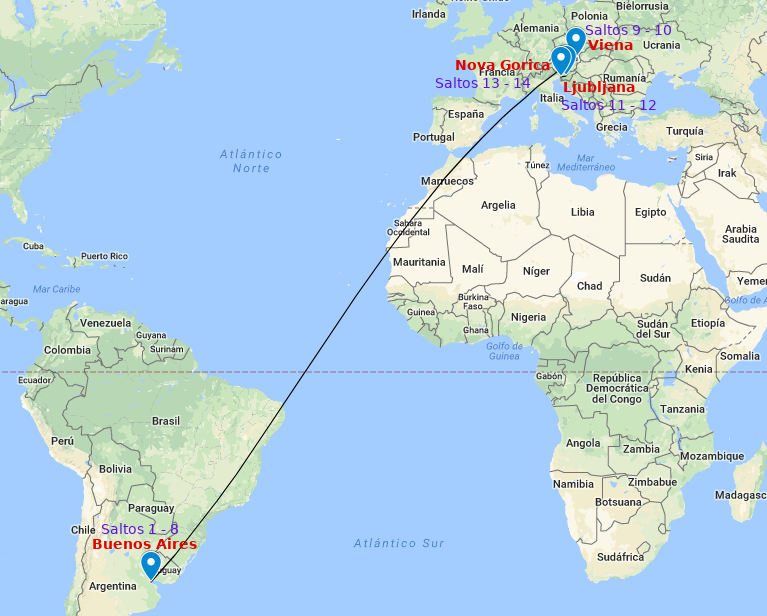
\includegraphics[width=\textwidth]{ljubljana.png}
\caption{Mapa de resultados para la Universidad de Ljubljana.}
\label{mapa3}
\end{figure}

En la figura \ref{diff3} vemos las diferencias de RTT por cada par de saltos. Observamos que algunos valores son negativos y que parece haber un máximo en el salto 7.

\begin{figure}[H]
\centering
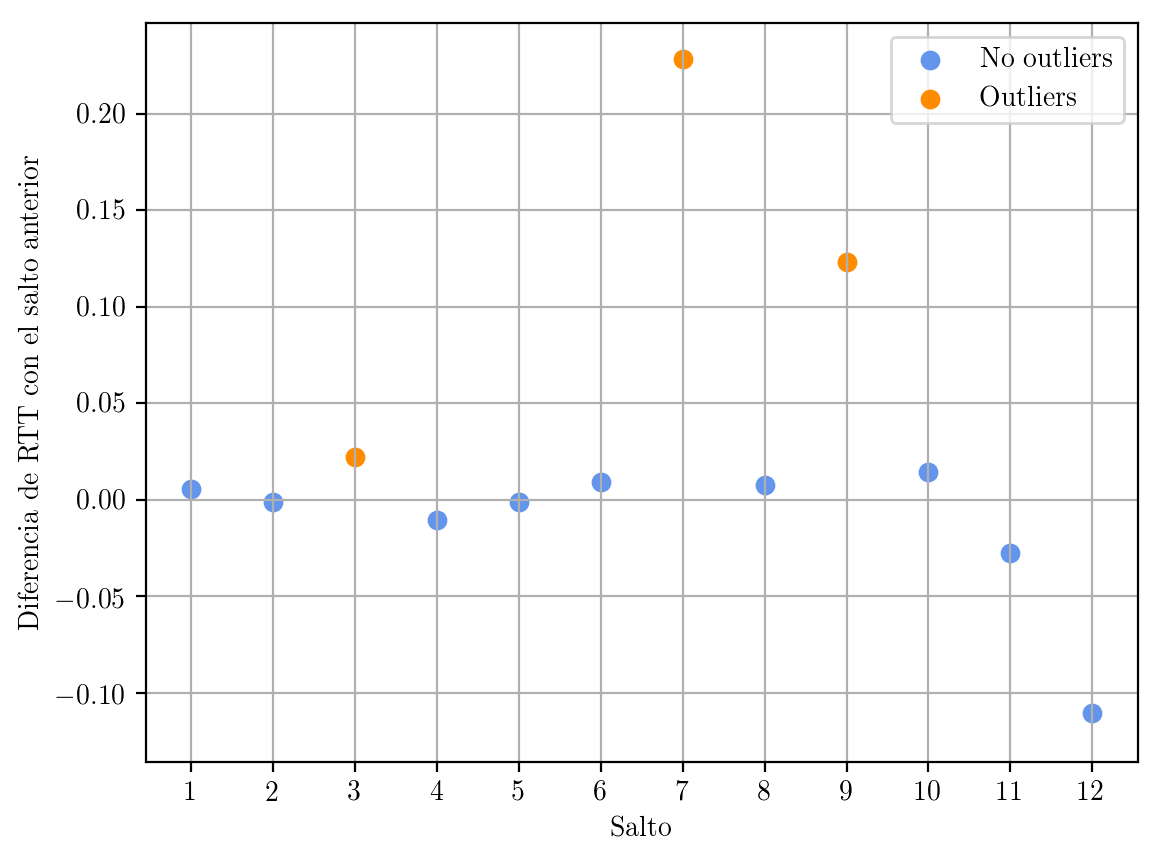
\includegraphics[width=0.6\textwidth]{ljubljana1.png}
\caption{Gráfico de diferencias de RTT en función de cada salto.}
\label{diff3}
\end{figure}

En la figura \ref{sdev3} observamos una dispersión muy grande de los puntos, lo que coincide con la gran cantidad de outliers encontrada.

\begin{figure}[H]
\centering
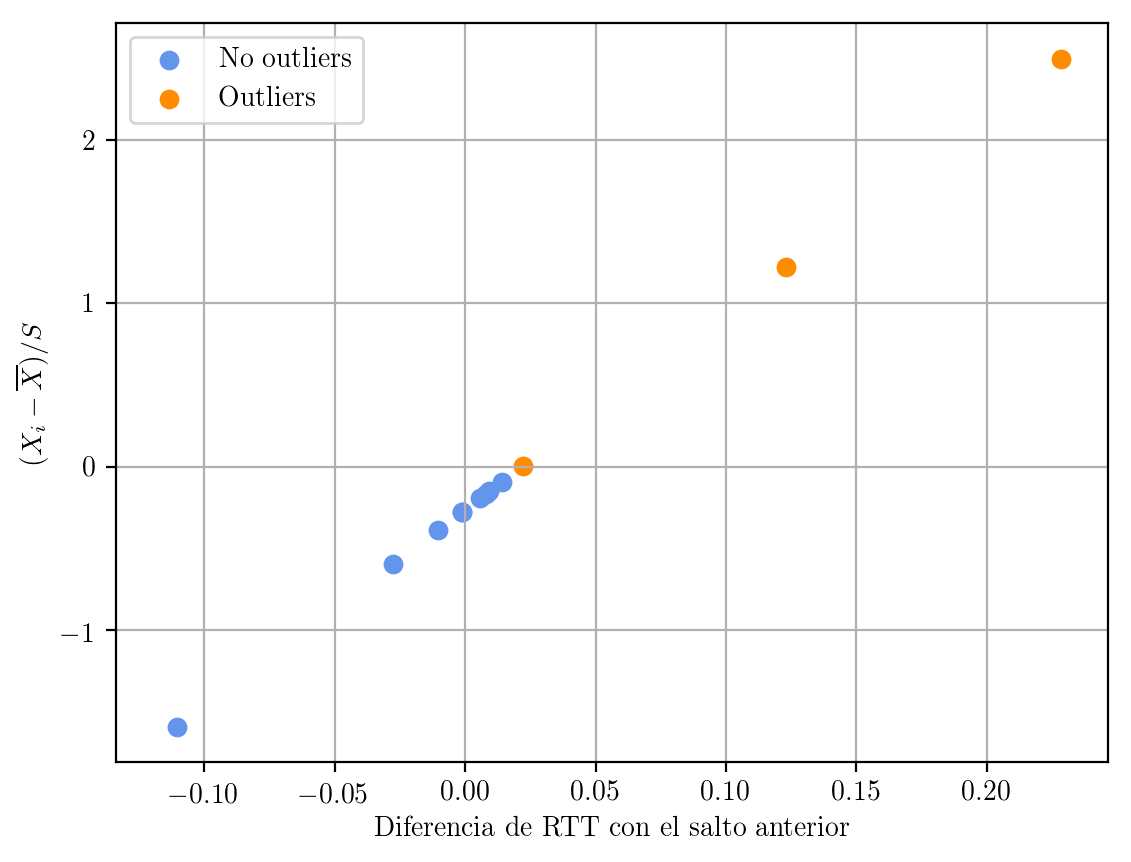
\includegraphics[width=0.6\textwidth]{ljubljana2.png}
\caption{Gráfico de $\frac{X_i - \bar{X}}{S}$ en función de las diferencias de RTT.}
\label{sdev3}
\end{figure}